% id: 0435
% book: RPM 중3-2 수학 · 04 원주각
% section: 유형 08 원주각의 크기와 호의 길이 (3)
% figure: crop:fig-0435.png
% answer: $56^\circ$
% answer_source: 답지
% variant_level: 0 (원본 전사)
% 이 파일은 build.mjs 가 items.json 에서 만든다. 고칠 때는 items.json 을 고친다.
\smash{\raisebox{4.5mm}{\dmkichul{서술형}}}
\noindent\begin{minipage}[t]{0.58\linewidth}\vspace{0pt}\raggedright 오른쪽 그림에서 점~$\pt{P}$는 두 현~$\pt{AC}$, $\pt{BD}$의 교점이다. $\arc{AB}$의 길이는 원주의 $\dfrac{1}{9}$이고 $\arc{CD}$의 길이는 원주의 $\dfrac{1}{5}$일 때, $\angle\pt{CPD}$의 크기를 구하시오.\end{minipage}\hfill\begin{minipage}[t]{0.4\linewidth}\vspace{0pt}\centering \setlength{\dmfigw}{75.0pt}\ifdim\dmfigw>\linewidth\setlength{\dmfigw}{\linewidth}\fi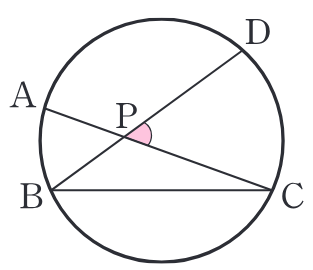
\includegraphics[width=\dmfigw]{figures/fig-0435.png}\end{minipage}\par
